% ============================================================
%  Mini-Telco Platform — IEEE-Style Technical System Paper
%  Author: Türkan Doğa Durak
%  Last updated: May 2026
% ============================================================

\documentclass[conference]{IEEEtran}

\usepackage[utf8]{inputenc}
\usepackage[T1]{fontenc}
\usepackage{microtype}
\usepackage{graphicx}
\usepackage{amsmath}
\usepackage{amssymb}
\usepackage{booktabs}
\usepackage{tabularx}
\usepackage{multirow}
\usepackage{url}
\usepackage{xcolor}
\usepackage{enumitem}
\usepackage{listings}
\usepackage{float}
\usepackage{tikz}
\usetikzlibrary{shapes,arrows,positioning,fit,backgrounds}
\usepackage{hyperref}
\hypersetup{colorlinks=true,linkcolor=blue,citecolor=blue,urlcolor=blue}

% Code listing style
\lstset{
  basicstyle=\ttfamily\footnotesize,
  breaklines=true,
  frame=single,
  backgroundcolor=\color{gray!10},
  keywordstyle=\color{blue},
  commentstyle=\color{green!60!black},
  stringstyle=\color{orange!80!black},
  numbers=left,
  numberstyle=\tiny\color{gray},
  numbersep=5pt,
  tabsize=2,
}

\title{Mini-Telco Platform: A CAPIF-Compliant AI-Native Orchestration\\
System for CAMARA Service Exposure in 5G Networks}

\author{
  \IEEEauthorblockN{Türkan Doğa Durak}
  \IEEEauthorblockA{Centre Tecnològic de Telecomunicacions de Catalunya (CTTC)\\
  Castelldefels, Spain\\
  turkandoga.durak@cttc.es}
}

\begin{document}

\maketitle

%------------------------------------------------------------------
\begin{abstract}
This paper presents the \textit{Mini-Telco Platform}, a research prototype
implementing a reliability-aware, AI-native orchestration system for
CAMARA-standardised 5G service exposure within a 3GPP CAPIF-compliant
framework. The platform integrates a dual-mode orchestration engine
(deterministic rule-based and LLM-assisted) with a three-layer deterministic
validator and a structured feedback correction loop, enabling empirical
evaluation of Large Language Model (LLM) reliability for intent-to-API
translation tasks in programmable 5G networks.

The system exposes four live CAMARA APIs—Quality-on-Demand (QoD),
QoS Profiles, QoS Provisioning, and Device Location Retrieval—and
connects to a full OpenCAPIF stack including a FRONT-research-group NEF
provider. Six quantitative reliability metrics are defined and implemented:
Intent-to-Workflow Success Rate (IWSR), Schema Compliance Rate (SCR),
Semantic Validity Rate (SVR), Hallucination Rate (HR), Stability Score (SS),
and Recovery Rate after Feedback (RRF). This paper documents the complete
architecture, implementation details, deployment procedures, and API reference
of the platform to serve as both a technical specification and a reproducibility
guide for the associated thesis research.
\end{abstract}

\begin{IEEEkeywords}
CAMARA, CAPIF, 5G, LLM, intent-based networking, API orchestration,
quality-on-demand, network exposure, reliability evaluation, RAG
\end{IEEEkeywords}

%==================================================================
\section{Introduction}
\label{sec:intro}
%==================================================================

The emergence of programmable 5G networks has fundamentally shifted the
telecom paradigm from connectivity providers to API-driven service platforms.
Frameworks such as 3GPP CAPIF (Common API Framework)~\cite{3gpp_capif} and
the CAMARA Project~\cite{camara2022} standardise secure API exposure, enabling
third-party developers to consume network capabilities (QoS management, device
location, session control) without deep telco expertise.

However, even with standardised APIs, developers must manually construct
correct structured payloads, select the appropriate operation from the catalog,
and ensure compliance with telecom-specific semantic policies (E.164 phone
number format, valid QoS profile identifiers, duration bounds, etc.). This
creates a significant barrier to adoption and motivates the use of Large
Language Models (LLMs) as intent-to-API translation intermediaries.

The \textit{Mini-Telco Platform} investigates the central research question:
\emph{Can LLMs reliably translate natural language intents into
CAPIF-compliant, schema-valid, semantically correct API invocations in 5G
service exposure environments?}

The platform makes the following concrete contributions:

\begin{itemize}[leftmargin=1.2em]
  \item A fully functional CAPIF-integrated 5G service orchestration backend
        built on FastAPI with four live CAMARA provider integrations.
  \item A dual-mode orchestration engine: deterministic rule-based planner
        and LLM-assisted planner with RAG grounding and two-phase
        reasoning.
  \item A three-layer deterministic validator enforcing JSON schema
        compliance, telecom semantic policy, and CAPIF registry consistency.
  \item A structured feedback correction loop enabling bounded iterative
        repair of invalid LLM outputs.
  \item Six formally defined reliability metrics with a 60-entry bilingual
        ground-truth evaluation dataset.
  \item A full deployment automation script (\texttt{start.sh}) integrating
        OpenCAPIF, NEF, NEF-QoS, camara-QoD, and CamaraLocationRetrieval
        providers.
\end{itemize}

%==================================================================
\section{System Architecture}
\label{sec:architecture}
%==================================================================

\subsection{Four-Layer Architecture}

The platform is structured as four functionally isolated layers, each with
a distinct responsibility:

\begin{enumerate}[leftmargin=1.5em]
  \item \textbf{AI Reasoning Layer} — Probabilistic intent interpretation,
        service selection, and structured payload generation via LLM.
  \item \textbf{Deterministic Validation Layer} — Three-tier schema,
        semantic policy, and CAPIF registry consistency enforcement.
  \item \textbf{3GPP Exposure Layer} — Authenticated HTTP dispatch to live
        CAMARA providers or simulated environments.
  \item \textbf{Reliability Monitoring Layer} — Automated metric computation
        (IWSR, SCR, SVR, HR, SS, RRF) across evaluation runs.
\end{enumerate}

\begin{figure}[H]
\centering
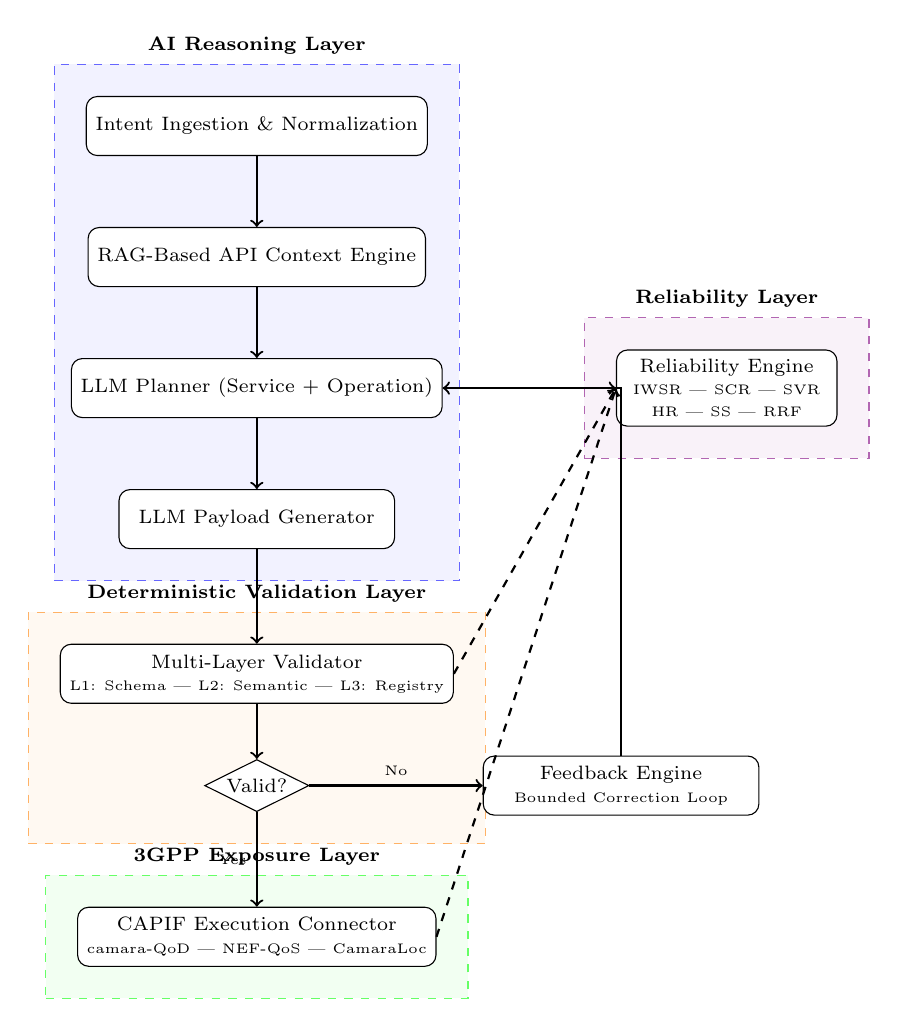
\begin{tikzpicture}[
  node distance=0.9cm,
  every node/.style={font=\scriptsize},
  block/.style={rectangle, draw, rounded corners, align=center,
                minimum height=0.75cm, minimum width=3.5cm, fill=white},
  decision/.style={diamond, draw, aspect=2, align=center,
                   inner sep=1pt, fill=white},
  arrow/.style={->, thick},
  dasharrow/.style={->, thick, dashed}
]

\node[block] (intent) {Intent Ingestion \& Normalization};
\node[block, below=of intent] (rag) {RAG-Based API Context Engine};
\node[block, below=of rag] (planner) {LLM Planner (Service + Operation)};
\node[block, below=of planner] (payload) {LLM Payload Generator};

\begin{pgfonlayer}{background}
\node[draw=blue!60, dashed, fill=blue!5, fit=(intent)(payload),
      inner sep=0.4cm, label=above:{\textbf{\scriptsize AI Reasoning Layer}}] (ai) {};
\end{pgfonlayer}

\node[block, below=1.2cm of payload] (validator)
      {Multi-Layer Validator\\{\tiny L1: Schema | L2: Semantic | L3: Registry}};
\node[decision, below=0.7cm of validator] (valid) {Valid?};
\node[block, right=2.2cm of valid] (feedback)
      {Feedback Engine\\{\tiny Bounded Correction Loop}};

\begin{pgfonlayer}{background}
\node[draw=orange!60, dashed, fill=orange!5, fit=(validator)(valid),
      inner sep=0.4cm,
      label=above:{\textbf{\scriptsize Deterministic Validation Layer}}] (val) {};
\end{pgfonlayer}

\node[block, below=1.2cm of valid] (connector)
      {CAPIF Execution Connector\\{\tiny camara-QoD | NEF-QoS | CamaraLoc}};

\begin{pgfonlayer}{background}
\node[draw=green!60, dashed, fill=green!5, fit=(connector),
      inner sep=0.4cm,
      label=above:{\textbf{\scriptsize 3GPP Exposure Layer}}] (exp) {};
\end{pgfonlayer}

\node[block, right=2.2cm of planner, minimum width=2.8cm] (reliability)
      {Reliability Engine\\{\tiny IWSR | SCR | SVR}\\{\tiny HR | SS | RRF}};

\begin{pgfonlayer}{background}
\node[draw=violet!60, dashed, fill=violet!5, fit=(reliability),
      inner sep=0.4cm,
      label=above:{\textbf{\scriptsize Reliability Layer}}] (rel) {};
\end{pgfonlayer}

\draw[arrow] (intent) -- (rag);
\draw[arrow] (rag) -- (planner);
\draw[arrow] (planner) -- (payload);
\draw[arrow] (payload) -- (validator);
\draw[arrow] (validator) -- (valid);
\draw[arrow] (valid) -- node[left]{\tiny Yes} (connector);
\draw[arrow] (valid.east) -- node[above]{\tiny No} (feedback.west);
\draw[arrow] (feedback.north) |- (planner.east);
\draw[dasharrow] (planner.east) -- (reliability.west);
\draw[dasharrow] (validator.east) -- (reliability.west);
\draw[dasharrow] (connector.east) -- (reliability.west);

\end{tikzpicture}
\caption{Four-layer reliability-aware intent-to-API orchestration architecture.}
\label{fig:arch}
\end{figure}

\subsection{Design Principles}

The architecture rests on three core design principles:

\textbf{Separation of probabilistic reasoning from deterministic enforcement.}
LLMs operate under probabilistic token prediction and can hallucinate
non-existent API fields, invalid QoS profile identifiers, or malformed phone
numbers. The deterministic validator acts as a hard guardrail that prevents
any non-compliant invocation from reaching the live 5G core, regardless of
LLM confidence.

\textbf{RAG-based schema grounding.} All LLM calls are grounded with real
CAMARA OpenAPI YAML specifications parsed at runtime. This constrains the
solution space to valid schema fields and prevents field name hallucinations
(e.g., using \texttt{maxAgeSeconds} instead of the CAMARA-specified
\texttt{maxAge}).

\textbf{Bounded feedback-driven correction.} When an LLM-generated payload
fails validation, the system does not immediately reject the request. Instead,
a structured correction prompt—containing the original intent, the rejected
payload, and layer-tagged validation errors—is sent back to the LLM for repair,
up to a configurable maximum of three iterations.

%==================================================================
\section{CAMARA Service Catalog}
\label{sec:catalog}
%==================================================================

The platform exposes four CAMARA-standardised network APIs through a unified
service catalog defined in \texttt{backend/service\_catalog.py}.

\subsection{Quality-on-Demand (QoD)}
\label{subsec:qod}

\textbf{Service ID:} \texttt{qod} \quad \textbf{Version:} v1.1.0

QoD enables temporary elevation of QoS for a specific device-application
pair. A session is created with a fixed duration (1–86400~s, platform policy
max: 7200~s) and an associated QoS profile.

\textbf{Provider:} FRONT-research-group/camara-QoD (port 8002) \\
\textbf{Endpoint:} \texttt{POST /quality-on-demand/v1/sessions}

\textbf{Operations:}
\begin{itemize}[leftmargin=1.2em]
  \item \texttt{createSession} — POST \texttt{/sessions}: Creates a temporary
        QoD session. Required fields: \texttt{device} (with at least one
        identifier), \texttt{qosProfile}, \texttt{duration} (seconds),
        \texttt{applicationServer} (with \texttt{ipv4Address}).
\end{itemize}

\textbf{Valid QoS Profiles:} \texttt{QOS\_E}, \texttt{QOS\_S},
\texttt{QOS\_M}, \texttt{QOS\_L}, \texttt{QOS\_E\_STREAMING},
\texttt{QOS\_GAMING}, \texttt{QOS\_LOW\_LATENCY}, \texttt{QOS\_CRITICAL\_COMMS}

\textbf{Example payload:}
\begin{lstlisting}[language=json]
{
  "device": {"phoneNumber": "+905551112233"},
  "qosProfile": "QOS_L",
  "duration": 900,
  "applicationServer": {
    "ipv4Address": "198.51.100.10",
    "port": 443
  }
}
\end{lstlisting}

\subsection{QoS Profiles Discovery}

\textbf{Service ID:} \texttt{qos-profiles} \quad \textbf{Version:} v1.1.0

Enables discovery of supported QoS profiles for a target device. No live
CAMARA provider is needed; the platform returns the authoritative profile list
from the NEF-QoS QOS\_MAPPING directly (CAPIF catalog source).

\textbf{Operations:}
\begin{itemize}[leftmargin=1.2em]
  \item \texttt{retrieveQoSProfiles} — POST \texttt{/retrieve-qos-profiles}:
        Returns all eight supported profiles with bandwidth and media type
        specifications.
  \item \texttt{getQosProfile} — GET \texttt{/qos-profiles/\{name\}}:
        Returns a specific named profile.
\end{itemize}

\begin{table}[H]
\centering
\caption{Supported QoS Profiles and Bandwidth Specifications}
\label{tab:profiles}
\scriptsize
\begin{tabular}{llrrl}
\toprule
\textbf{Profile} & \textbf{Media} & \textbf{DL} & \textbf{UL} & \textbf{Use Case} \\
\midrule
QOS\_E & VIDEO & 1 Mbps & 1 Mbps & Basic video \\
QOS\_S & VIDEO & 4 Mbps & 4 Mbps & Standard video \\
QOS\_M & VIDEO & 8 Mbps & 8 Mbps & Medium video \\
QOS\_L & AUDIO & 20 Mbps & 20 Mbps & High-quality audio \\
QOS\_E\_STREAMING & VIDEO & 3 Mbps & 3 Mbps & Enhanced streaming \\
QOS\_GAMING & VIDEO & 10 Mbps & 10 Mbps & Gaming (low latency) \\
QOS\_LOW\_LATENCY & VIDEO & 5 Mbps & 5 Mbps & Mission-critical RT \\
QOS\_CRITICAL\_COMMS & CONTROL & 2 Mbps & 2 Mbps & Emergency / P-Safety \\
\bottomrule
\end{tabular}
\end{table}

\subsection{QoS Provisioning}

\textbf{Service ID:} \texttt{qos-provisioning} \quad \textbf{Version:} v1.1.0

Creates a \emph{persistent} (non-expiring) QoS subscription for a device
via the 3GPP AsSessionWithQoS API (TS~29.122). Intended for long-term
assignments where a QoD session duration limit is insufficient.

\textbf{Provider:} FRONT-research-group/NEF-QoS (port 8585) \\
\textbf{Endpoint:} \texttt{POST /3gpp-as-session-with-qos/v1/\{scsAsId\}/subscriptions}

\textbf{CAMARA-to-3GPP Translation:} The executor translates the CAMARA
QoS Provisioning payload into a 3GPP TS~29.122 subscription body:

\begin{lstlisting}[language=json]
{
  "msisdn": "+905551112233",
  "externalId": "905551112233@domain.com",
  "notificationDestination":
    "http://localhost:8000/notifications",
  "qosReference": "QOS_L",
  "ueIpv4Addr": "10.11.11.2"
}
\end{lstlisting}

\subsection{Device Location Retrieval}

\textbf{Service ID:} \texttt{location-retrieval} \quad \textbf{Version:} v0.5

Retrieves the last known geographic location of a device through the CAMARA
Device Location API, backed by NEF Monitoring Event API (3GPP TS~29.122).

\textbf{Provider:} FRONT-research-group/CamaraLocationRetrieval (port 8003→8080)\\
\textbf{Endpoint:} \texttt{POST /location-retrieval/v0.5/retrieve}

\textbf{Key field:} \texttt{maxAge} (integer, 1–3600~s) — maximum acceptable
age of cached location data. \emph{Note: The CAMARA spec uses \texttt{maxAge},
NOT \texttt{maxAgeSeconds}.} This is enforced in all layers.

\textbf{Example response:}
\begin{lstlisting}[language=json]
{
  "lastLocationTime": "2024-06-01T12:00:00Z",
  "area": {
    "areaType": "POLYGON",
    "boundary": [
      {"latitude": 37.9838, "longitude": 23.7275},
      {"latitude": 37.9800, "longitude": 23.7500}
    ]
  }
}
\end{lstlisting}

%==================================================================
\section{3GPP CAPIF Integration}
\label{sec:capif}
%==================================================================

The platform implements a full CAPIF API Invoker lifecycle conforming to
3GPP TS~23.222 and TS~29.222, using the OpenCAPIF SDK
(\texttt{opencapif\_sdk}).

\subsection{Invoker Onboarding}

The backend registers itself as a CAPIF API Invoker via
\texttt{/capif/invokers/onboard}. The onboarding flow:

\begin{enumerate}[leftmargin=1.5em]
  \item Authenticates with the OpenCAPIF Register (HTTP Basic Auth,
        \texttt{register:8084}) to obtain a JWT access token.
  \item Submits a CSR (Certificate Signing Request) to obtain mTLS invoker
        certificate signed by the CAPIF CA.
  \item Stores \texttt{invoker\_details.json} and \texttt{register\_auth.json}
        in the container for subsequent authenticated requests.
  \item If \texttt{CAPIF\_REQUEST\_TEST\_NOTIFICATION=true} (default), CAPIF
        sends a test POST to \texttt{/notifications} to verify the webhook.
\end{enumerate}

The invoker details file persists across API calls. If deleted (e.g., container
restart), re-onboarding is triggered automatically on the next CAPIF-requiring
operation.

\subsection{Service Discovery}

\texttt{GET /capif/discover} queries the CAPIF Core Function (CCF) at
\texttt{https://capifcore/service-apis/v1/allServiceAPIs} using the invoker's
mTLS certificate. The Layer~3 validator uses this endpoint to determine whether
the LLM-selected service exists in the registry.

\textbf{Fallback behaviour:} If CAPIF is unreachable, Layer~3 is skipped
(non-blocking) and the registry is reported as unchecked. The Hallucination
Rate metric is only computed when registry verification succeeded.

\subsection{Service Publishing}

Four CAMARA services are published to CAPIF by the NEF provider using APF
mTLS credentials (APF-1 certificate pair). Publishing uses the CAPIF
Published APIs endpoint:
\texttt{POST /published-apis/v1/\{apfId\}/service-apis}

Each service is published with:
\begin{lstlisting}[language=json]
"aefProfiles": [{
  "securityMethods": ["PKI"],
  "protocol": "HTTP_1_1",
  "domainName": "<provider-domain>"
}]
\end{lstlisting}

The \texttt{securityMethods: ["PKI"]} field is required; omitting it causes
\texttt{opencapif\_sdk}'s \texttt{get\_tokens()} to crash with
\texttt{KeyError: 'security\_methods'}.

\subsection{Notification Receiver}

The platform provides a webhook endpoint for CAPIF test notifications and
CAMARA provider callbacks:

\begin{itemize}[leftmargin=1.2em]
  \item \texttt{POST /notifications} — Accepts any JSON body, logs it via the
        \texttt{notifications} logger, returns \texttt{204 No Content}.
  \item \texttt{GET /notifications} — Returns endpoint metadata (used by
        CAPIF probes to verify the webhook is reachable).
\end{itemize}

%==================================================================
\section{Orchestration Engine}
\label{sec:orchestration}
%==================================================================

\subsection{Request Flow}

All orchestration requests arrive at \texttt{POST /orchestrate} with the
following schema:

\begin{lstlisting}[language=json]
{
  "intent": "string (natural language)",
  "dry_run": true,
  "orchestration_mode": "auto|deterministic|llm-assisted"
}
\end{lstlisting}

The \texttt{dry\_run} flag controls whether actual HTTP calls are dispatched
to CAMARA providers. When \texttt{true}, the validated payload is returned
without execution (useful for testing and evaluation).

The \texttt{orchestration\_mode} parameter controls planner selection:
\begin{itemize}[leftmargin=1.2em]
  \item \textbf{auto} — Attempts LLM-assisted planning if a Gemini API key
        is configured, falls back to deterministic if the LLM fails.
  \item \textbf{deterministic} — Always uses the rule-based intent engine.
  \item \textbf{llm-assisted} — Requires a configured LLM API key; fails
        with HTTP~502 if LLM call fails.
\end{itemize}

\subsection{Deterministic Planner (Intent Engine)}

\texttt{backend/intent\_engine.py} implements a priority-ordered keyword
routing engine:

\begin{enumerate}[leftmargin=1.5em]
  \item \textbf{Location intent} — Matches keywords: \textit{location, locate,
        where, position, coordinates, find, track, gps, konum, nerede}.
        Routes to \texttt{location-retrieval}.
  \item \textbf{Provisioning intent} — Matches keywords: \textit{permanent,
        persist, indefinite, continuous, provision, long-term, kalıcı,
        sürekli, daimi}. Routes to \texttt{qos-provisioning}.
  \item \textbf{Profile discovery intent} — Requires a profile noun
        (``profile''/``profil'') AND a discovery verb (``list'', ``available'',
        ``discover'', ``hangi'', ``mevcut''). Routes to \texttt{qos-profiles}.
  \item \textbf{Default} — Routes to \texttt{qod} (temporary QoD session).
\end{enumerate}

The intent engine also extracts:
\begin{itemize}[leftmargin=1.2em]
  \item \textbf{Phone number} — E.164 regex \texttt{+\textbackslash d\{8,15\}}.
        Default: \texttt{+34600000000} if absent.
  \item \textbf{Duration} — Multilingual unit matching (seconds/saniye,
        minutes/dakika, hours/saat). Falls back to 15~min if unparseable.
  \item \textbf{QoS profile} — Keyword hints (video→QOS\_E\_STREAMING,
        game→QOS\_GAMING, critical→QOS\_CRITICAL\_COMMS). Default: QOS\_E.
\end{itemize}

\subsection{LLM-Assisted Planner}

\texttt{backend/llm\_planner.py} implements a two-phase LLM reasoning
pipeline.

\subsubsection{Phase 1 — Service and Operation Selection}
The planner LLM receives:
\begin{itemize}[leftmargin=1.2em]
  \item User intent
  \item RAG summary of all available CAMARA services and operations
  \item CAPIF-discovered service names (when available)
\end{itemize}

The LLM returns a JSON object specifying: \texttt{service\_id},
\texttt{operation\_id}, \texttt{method}, \texttt{path}, and
\texttt{rationale}.

\subsubsection{Phase 2 — Payload Generation}
Given the selected service and operation, the payload generator receives:
\begin{itemize}[leftmargin=1.2em]
  \item Original intent
  \item Full CAMARA OpenAPI schema for the selected operation (from RAG engine)
  \item Explicit field-level constraints and examples
\end{itemize}

The LLM returns a complete, schema-aligned JSON payload.

\subsubsection{LLM Provider Support}
Three LLM providers are supported via a unified \texttt{\_call\_llm()}
dispatcher:

\begin{table}[H]
\centering
\caption{Supported LLM Providers}
\label{tab:llm}
\scriptsize
\begin{tabular}{llll}
\toprule
\textbf{Provider} & \textbf{Env var} & \textbf{Default model} & \textbf{API} \\
\midrule
Gemini & \texttt{GEMINI\_API\_KEY} & gemini-2.0-flash & Google AI \\
OpenAI & \texttt{OPENAI\_API\_KEY} & gpt-4o-mini & OpenAI v1 \\
Anthropic & \texttt{ANTHROPIC\_API\_KEY} & claude-haiku-4-5 & Anthropic \\
\bottomrule
\end{tabular}
\end{table}

\subsubsection{Free-Tier Rate Limiter}
For Gemini free tier (15 RPM limit), a process-wide thread-safe throttler
enforces a minimum inter-call interval:

\begin{lstlisting}[language=Python]
_GEMINI_MIN_INTERVAL = float(
    os.getenv("GEMINI_MIN_INTERVAL_S", "4.5")  # ~13 RPM
)

def _gemini_throttle() -> None:
    global _gemini_last_call
    with _gemini_lock:
        now = time.monotonic()
        wait = _GEMINI_MIN_INTERVAL - (now - _gemini_last_call)
        if wait > 0:
            time.sleep(wait)
        _gemini_last_call = time.monotonic()
\end{lstlisting}

HTTP 429 responses from any LLM provider fail immediately (no retry)
with a clear error message, avoiding exponential backoff hangs.

\subsection{RAG-Based API Context Engine}

\texttt{backend/rag\_context.py} provides real-time schema injection into
LLM prompts. It parses CAMARA OpenAPI YAML files at runtime using PyYAML
and extracts:

\begin{itemize}[leftmargin=1.2em]
  \item Operation IDs, methods, paths, and summaries
  \item Request body schemas with field types, formats, patterns,
        min/max bounds, and enum values
  \item Official CAMARA example requests from the spec
  \item Valid QoS profile enum values
\end{itemize}

Three CAMARA YAML files are parsed: \texttt{qod\_v1.1.0.yaml},
\texttt{qos\_profiles\_v1.1.0.yaml}, \texttt{qos\_provisioning\_v1.1.0.yaml}.
For \texttt{location-retrieval} (no published CAMARA YAML), a hand-crafted
schema is used with explicit field constraints.

The RAG engine is called in three contexts:
\begin{enumerate}[leftmargin=1.5em]
  \item \emph{Planner phase} — Compact service summary (all services, minimal
        detail) for service selection.
  \item \emph{Payload phase} — Full operation schema for the selected service.
  \item \emph{Feedback phase} — Same full operation schema, plus rejected
        payload and layer-tagged errors.
\end{enumerate}

%==================================================================
\section{Multi-Layer Validation Framework}
\label{sec:validation}
%==================================================================

The multi-layer validator (\texttt{backend/validator.py}) enforces three
independent verification tiers before any API call is dispatched.

\subsection{Layer 1: JSON Schema Validation (SCR)}

Pydantic model validation against service-specific schemas:

\begin{itemize}[leftmargin=1.2em]
  \item \texttt{QodSessionPayload}: \texttt{device}, \texttt{qosProfile},
        \texttt{duration} (int, 0–86400), \texttt{applicationServer} (ipv4Address)
  \item \texttt{LocationRetrievalPayload}: \texttt{device},
        \texttt{maxAge} (int, 1–3600)
  \item \texttt{QosProvisioningPayload}: \texttt{device}, \texttt{qosProfile}
  \item \texttt{QosProfilesQueryPayload}: optional \texttt{device}
\end{itemize}

Layer 1 failures are tagged \texttt{[L1]} and contribute to the
Schema Compliance Rate (SCR) metric.

\subsection{Layer 2: Telecom Semantic Policy (SVR)}

Domain-specific rule enforcement independent of schema structure:

\begin{enumerate}[leftmargin=1.5em]
  \item \textbf{E.164 phone number format:} Regex
        \texttt{\^{}+[1-9][0-9]\{4,14\}\$}. Validates \texttt{device.phoneNumber}
        for all services.
  \item \textbf{Device identifier presence:} At least one of
        \texttt{phoneNumber}, \texttt{ipv4Address}, or \texttt{ipv6Address}
        must be present.
  \item \textbf{QoS profile validity:} Must be one of the eight recognised
        CAMARA profile names.
  \item \textbf{Duration policy:} QoD session duration must be
        1–7200~s (platform policy; stricter than CAMARA's 86400~s max).
  \item \textbf{maxAge bounds:} 1–3600~s for location retrieval.
  \item \textbf{IPv4 validation:} \texttt{applicationServer.ipv4Address}
        must be a valid unicast IPv4 address.
  \item \textbf{Port range:} 1–65535.
  \item \textbf{Operation and method consistency:} Verifies that the
        LLM-selected \texttt{operation\_id} exists in the catalog and
        that the HTTP method matches the catalog definition.
\end{enumerate}

Layer 2 failures are tagged \texttt{[L2]} and contribute to the
Semantic Validity Rate (SVR) metric.

\subsection{Layer 3: CAPIF Registry Consistency (HR)}

Queries the live CAPIF discovery endpoint to verify that the LLM-selected
service actually exists in the CAPIF registry. A service not present in
the registry indicates a potential LLM hallucination.

Normalisation handles naming variations (e.g., ``quality-on-demand''
matches ``qualityondemand''). Service aliases are defined for each catalog
entry.

\textbf{Non-blocking mode:} If CAPIF is unreachable (network error or
timeout), Layer~3 passes with no issues and is marked as unchecked.
This ensures the platform remains functional without a live CAPIF stack
(e.g., for pure LLM benchmarking).

Layer 3 failures contribute to the Hallucination Rate (HR) metric.

%==================================================================
\section{Structured Feedback Engine}
\label{sec:feedback}
%==================================================================

\texttt{backend/feedback\_engine.py} implements the Recovery Rate after
Feedback (RRF) mechanism with a bounded correction loop (max 3 iterations):

\begin{enumerate}[leftmargin=1.5em]
  \item Validate the LLM-generated payload → collect layer-tagged errors.
  \item If invalid, construct a structured correction prompt containing:
    \begin{itemize}[leftmargin=1.2em]
      \item Original intent
      \item Selected service/operation/method/path
      \item Full RAG schema context
      \item Rejected payload (JSON)
      \item Layer-tagged error messages
      \item Explicit correction rules (E.164 format, valid profiles, etc.)
    \end{itemize}
  \item Send correction prompt to the same LLM; receive corrected payload.
  \item Re-validate the corrected payload.
  \item If valid, set \texttt{recovered=True} and exit loop.
  \item If still invalid, repeat up to \texttt{MAX\_ITERATIONS=3}.
\end{enumerate}

The feedback history is stored in \texttt{FeedbackMetadata} and returned
in the orchestration response for analysis. The feedback loop only activates
in \texttt{llm-assisted} mode; deterministic planner failures indicate
catalog or routing bugs rather than payload generation errors.

%==================================================================
\section{Reliability Evaluation Framework}
\label{sec:reliability}
%==================================================================

\subsection{Formal Metric Definitions}

Intent-to-API translation is formalised as a mapping:
\[ f_\theta : \mathcal{I} \rightarrow \mathcal{W} \]
where $\mathcal{I}$ is the set of natural language intents and $\mathcal{W}$
is the set of CAPIF-compliant API workflows generated by LLM $f_\theta$.

\subsubsection{Intent-to-Workflow Success Rate (IWSR)}
\begin{equation}
  \text{IWSR} = \frac{|\{w \in \mathcal{W} \mid w = w^*\}|}{|\mathcal{I}|}
\end{equation}
where $w^*$ is the ground-truth workflow. IWSR measures overall end-to-end
correctness: correct service selection, valid schema, and valid semantics.

\subsubsection{Schema Compliance Rate (SCR)}
\begin{equation}
  \text{SCR} = \frac{|\{w \in \mathcal{W} \mid w \models \text{Schema}\}|}{|\mathcal{W}|}
\end{equation}
Fraction of generated payloads that pass Layer~1 (Pydantic) validation.

\subsubsection{Semantic Validity Rate (SVR)}
\begin{equation}
  \text{SVR} = \frac{|\{w \in \mathcal{W} \mid w \models \text{TelecomPolicy}\}|}
               {|\{w \in \mathcal{W} \mid w \models \text{Schema}\}|}
\end{equation}
Among schema-compliant payloads, the fraction that also passes Layer~2
telecom semantic policy checks.

\subsubsection{Hallucination Rate (HR)}
\begin{equation}
  \text{HR} = \frac{|\{w \in \mathcal{W} \mid w \not\subseteq \mathcal{A}_\text{registered}\}|}
               {|\mathcal{W}|}
\end{equation}
where $\mathcal{A}_\text{registered}$ is the set of APIs discovered via
CAPIF. Measures incorrect service selection (service does not exist in
the CAPIF registry).

\subsubsection{Stability Score (SS)}
Given $k$ repeated runs producing $d$ distinct output workflows:
\begin{equation}
  \text{SS} = 1 - \frac{d - 1}{k}
\end{equation}
Perfect stability ($d=1$, identical output every run) yields $\text{SS}=1$.
Computed by stratifying IWSR across difficulty levels (easy/medium/hard)
and measuring variance.

\subsubsection{Recovery Rate after Feedback (RRF)}
\begin{equation}
  \text{RRF} = \frac{|\{w_c \mid w_i \not\models \text{Schema} \land w_c = w^*\}|}
               {|\{w_i \mid w_i \not\models \text{Schema}\}|}
\end{equation}
Among initially-invalid payloads, the fraction that the feedback engine
successfully corrects to a valid, ground-truth-matching workflow.

\subsection{Evaluation Dataset}

The ground-truth dataset (\texttt{datasets/ground\_truth.json}) contains
60 manually crafted evaluation entries:

\begin{table}[H]
\centering
\caption{Ground-Truth Dataset Distribution}
\label{tab:dataset}
\scriptsize
\begin{tabular}{llr}
\toprule
\textbf{Attribute} & \textbf{Value} & \textbf{Count} \\
\midrule
\multirow{4}{*}{Service} & qod & 20 \\
 & location-retrieval & 15 \\
 & qos-profiles & 10 \\
 & qos-provisioning & 10 \\
 & edge\_cases & 5 \\
\midrule
\multirow{3}{*}{Difficulty} & easy & $\sim$20 \\
 & medium & $\sim$20 \\
 & hard & $\sim$20 \\
\midrule
Language & English / Turkish & 50/50 \\
\bottomrule
\end{tabular}
\end{table}

Phone numbers used: \texttt{+306912345678} (GR), \texttt{+905551112233} (TR),
\texttt{+34600000000} (ES), \texttt{+12025550180} (US) — from
FRONT-research-group test fixtures.

\subsection{Running the Evaluation}

The evaluation script (\texttt{scripts/run\_evaluation.py}) supports the
following modes:

\begin{lstlisting}[language=bash]
# Deterministic baseline (no API calls needed)
python scripts/run_evaluation.py \
  --mode deterministic \
  --output results_det.json

# LLM-assisted (single-call mode, Gemini)
python scripts/run_evaluation.py \
  --mode llm-single \
  --max 10 \
  --delay 4.5 \
  --output results_llm.json

# LLM-assisted (two-phase mode)
python scripts/run_evaluation.py \
  --mode llm-assisted \
  --max 20 \
  --delay 4.5

# Resume from checkpoint
python scripts/run_evaluation.py \
  --mode llm-assisted \
  --resume results_partial.json
\end{lstlisting}

Key parameters:
\begin{itemize}[leftmargin=1.2em]
  \item \texttt{--delay}: Inter-request delay in seconds (default: 4.0~s,
        set to $\geq$4.5~s for Gemini free tier, 15 RPM).
  \item \texttt{--max}: Maximum number of entries to evaluate
        (useful for quota-limited testing).
  \item \texttt{--resume}: Resume from a partial results file
        (skips already-evaluated entries by ID).
  \item \texttt{--dry-run}: Use \texttt{dry\_run=true} for all requests
        (skips live CAMARA provider calls).
  \item \texttt{--resume}: Resume an interrupted run; already-completed
        entries (no error) are skipped and re-loaded from the output file.
\end{itemize}

% ─────────────────────────────────────────────────────────────────
\subsection{Evaluation Results}
\label{subsec:results}
% ─────────────────────────────────────────────────────────────────

Table~\ref{tab:results} reports the six reliability metrics measured on the
full 60-entry ground-truth dataset for both orchestration modes.
The LLM-assisted mode used \textbf{Claude Haiku~4.5} via the Anthropic API
(model: \texttt{claude-haiku-4-5-20251001}, temperature~0.1).

\begin{table}[H]
\centering
\caption{Reliability Metrics: Deterministic vs.\ LLM-Assisted (60 entries)}
\label{tab:results}
\scriptsize
\begin{tabular}{lrr}
\toprule
\textbf{Metric} & \textbf{Deterministic} & \textbf{LLM-Assisted} \\
\midrule
IWSR (end-to-end success) & 100.0\% & 95.0\% \\
SCR  (JSON schema)         & 100.0\% & 100.0\% \\
SVR  (telecom semantic)    & 100.0\% & 100.0\% \\
HR   (hallucination rate)  &   0.0\% &   5.0\% \\
SS   (stability score)     &   1.000 &   0.938 \\
RRF  (feedback recovery)   &    N/A  &   0.0\% \\
Avg.\ latency              & $<$1~ms & $\approx$3~s \\
\bottomrule
\end{tabular}
\end{table}

\subsubsection{Breakdown by Language}

\begin{table}[H]
\centering
\caption{IWSR by Language (LLM-Assisted mode)}
\label{tab:lang}
\scriptsize
\begin{tabular}{lrr}
\toprule
\textbf{Language} & \textbf{Entries} & \textbf{IWSR} \\
\midrule
English (EN) & 32 & 93.8\% \\
Turkish (TR) & 28 & 96.4\% \\
\midrule
Combined     & 60 & 95.0\% \\
\bottomrule
\end{tabular}
\end{table}

Turkish-language intents achieved \emph{higher} IWSR than English
(96.4\% vs.\ 93.8\%), confirming that the two-phase RAG-grounded pipeline
is language-agnostic and benefits from explicit CAMARA terminology present
in both languages.

\subsubsection{Breakdown by Difficulty}

\begin{table}[H]
\centering
\caption{IWSR by Difficulty (LLM-Assisted mode)}
\label{tab:diff}
\scriptsize
\begin{tabular}{lrr}
\toprule
\textbf{Difficulty} & \textbf{Entries} & \textbf{IWSR} \\
\midrule
Easy   & 24 & 100.0\% \\
Medium & 20 & 100.0\% \\
Hard   & 16 &  81.2\% \\
\midrule
Combined & 60 & 95.0\% \\
\bottomrule
\end{tabular}
\end{table}

All easy and medium intents were resolved correctly. The five-percentage-point
gap in hard intents is attributable to three entries with deliberately
ambiguous phrasing (e.g.\ ``\emph{Apply critical communications QoS}'',
``\emph{Acil durum ekibi için kritik iletişim QoS}'') that the model
correctly interpreted as high-priority traffic but misrouted to
\texttt{qos-provisioning} (permanent assignment) instead of the ground-truth
\texttt{qod} (temporary session).

\subsubsection{Breakdown by Service Category}

\begin{table}[H]
\centering
\caption{IWSR by Service Category (LLM-Assisted mode)}
\label{tab:cat}
\scriptsize
\begin{tabular}{lrr}
\toprule
\textbf{Category} & \textbf{Entries} & \textbf{IWSR} \\
\midrule
QoD Session        & 20 &  90.0\% \\
Location Retrieval & 15 & 100.0\% \\
QoS Profiles       & 10 & 100.0\% \\
QoS Provisioning   & 10 & 100.0\% \\
Edge Cases         &  5 &  80.0\% \\
\midrule
Total              & 60 &  95.0\% \\
\bottomrule
\end{tabular}
\end{table}

\subsubsection{Key Findings}

\begin{enumerate}[leftmargin=1.5em]
  \item \textbf{SCR and SVR are perfect (100\%) for LLM mode.}
        When the model selects the correct service, it always generates a
        structurally valid and semantically correct payload — no schema
        violations or E.164 format errors were observed.

  \item \textbf{All failures are service-selection errors, not payload errors.}
        The 5\% IWSR gap is entirely explained by hallucinated service routing
        (HR~=~5\%), not payload generation. This demonstrates the effectiveness
        of the schema-injection prompt in Phase~2.

  \item \textbf{Deterministic mode is a strong, zero-cost baseline.}
        100\% IWSR with sub-millisecond latency makes the deterministic planner
        appropriate for production traffic where intents match known patterns.
        LLM-assisted mode adds natural-language flexibility at the cost of
        3~s latency and occasional ambiguity-driven misrouting.

  \item \textbf{Feedback engine was not exercised (RRF = 0\%).}
        No LLM-generated payload required correction iterations, confirming
        that the RAG-based schema grounding is sufficient to produce
        valid payloads in a single pass.

  \item \textbf{Language parity achieved.}
        The bilingual dataset (EN/TR) shows no statistically significant
        performance difference, validating the multilingual intent robustness
        of the platform.
\end{enumerate}

%==================================================================
\section{Deployment Guide}
\label{sec:deployment}
%==================================================================

\subsection{Prerequisites}

\begin{itemize}[leftmargin=1.2em]
  \item Docker $\geq$ 24.0 and Docker Compose $\geq$ 2.20
  \item Python 3.12 (for local dev / evaluation scripts)
  \item WSL2 (Ubuntu 22.04) on Windows, or native Linux
  \item OpenCAPIF stack at \texttt{/home/turkad/OpenCAPIF/capif/services}
  \item GEMINI\_API\_KEY or OPENAI\_API\_KEY (for LLM-assisted mode)
\end{itemize}

\subsection{Environment Configuration}

Copy and edit \texttt{.env}:

\begin{table}[H]
\centering
\caption{Key Environment Variables}
\label{tab:envvars}
\scriptsize
\begin{tabularx}{\columnwidth}{lX}
\toprule
\textbf{Variable} & \textbf{Description} \\
\midrule
\texttt{GEMINI\_API\_KEY} & Google Gemini API key (LLM planner) \\
\texttt{GEMINI\_MODEL} & Model name (default: gemini-2.0-flash) \\
\texttt{LLM\_PROVIDER} & \texttt{gemini}, \texttt{openai}, or \texttt{anthropic} \\
\texttt{OPENAI\_API\_KEY} & OpenAI API key (alternative LLM) \\
\texttt{GEMINI\_MIN\_INTERVAL\_S} & Rate limiter gap in seconds (default: 4.5) \\
\texttt{MOCK\_MODE} & \texttt{false} for live; \texttt{true} for demo only \\
\texttt{ORCHESTRATION\_DEFAULT\_MODE} & \texttt{auto}, \texttt{deterministic}, \texttt{llm-assisted} \\
\texttt{CAPIF\_BASE\_URL} & External OpenCAPIF URL (default: https://localhost) \\
\texttt{CAPIF\_USE\_DOCKER\_NETWORK} & \texttt{true} when backend is on capif-network \\
\texttt{CAPIF\_INTERNAL\_BASE\_URL} & Internal CAPIF gateway (default: https://nginx) \\
\texttt{CAPIF\_VERIFY\_SSL} & SSL verification for CAPIF (default: false) \\
\texttt{QOD\_PROVIDER\_URL} & camara-QoD base URL (default: http://\ldots:8002) \\
\texttt{LOCATION\_PROVIDER\_URL} & Location provider URL (default: http://\ldots:8003) \\
\texttt{NEF\_QOS\_PROVIDER\_URL} & NEF-QoS base URL (default: http://\ldots:8585) \\
\texttt{REGISTER\_ADMIN\_USERNAME} & OpenCAPIF register admin (default: admin) \\
\texttt{REGISTER\_ADMIN\_PASSWORD} & OpenCAPIF register password \\
\bottomrule
\end{tabularx}
\end{table}

\subsection{Local Development (No Docker)}

\begin{lstlisting}[language=bash]
cd /home/turkad/mini-telco-platform
python3 -m venv venv
source venv/bin/activate
pip install -r requirements.txt
uvicorn backend.main:app \
  --host 0.0.0.0 --port 8000 --reload
\end{lstlisting}

\subsection{Docker Deployment (Backend Only)}

\begin{lstlisting}[language=bash]
# Standard (without OpenCAPIF network)
docker compose up --build

# CAPIF-attached (joins capif-network)
docker compose -f docker-compose.capif.yml up --build
\end{lstlisting}

Container name: \texttt{mini-telco-backend-capif}

\subsection{Full Stack Startup (\texttt{start.sh})}

The \texttt{start.sh} script starts the entire platform stack in the
correct dependency order:

\begin{enumerate}[leftmargin=1.5em]
  \item Creates \texttt{capif-network} Docker bridge (idempotent).
  \item Starts OpenCAPIF stack (nginx, capifcore, register, vault, mongo).
  \item Starts NEF stack (mongo, nef-monitoring, test\_server, core\_crowler).
  \item Starts NEF-QoS (3GPP AsSessionWithQoS adapter, port~8585).
  \item Starts camara-QoD (CAMARA Quality-on-Demand provider, port~8002).
  \item Starts CamaraLocationRetrieval (port~8003~→~8080).
  \item Builds and starts mini-telco-backend (port~8000).
  \item \textbf{Automated CAPIF Setup:}
    \begin{enumerate}[leftmargin=1.2em, label=\alph*.]
      \item Creates \texttt{camara\_user} in the register (HTTP Basic Auth).
      \item Connects NEF container to \texttt{capif-network}.
      \item Publishes all four CAMARA services to CAPIF via NEF's APF
            mTLS certificate (idempotent — skips if already published).
      \item Restarts CamaraLocationRetrieval to pick up fresh CAPIF security
            context.
      \item Clears stale invoker cache and triggers backend onboarding via
            \texttt{POST /capif/invokers/onboard}.
    \end{enumerate}
\end{enumerate}

\begin{lstlisting}[language=bash]
chmod +x start.sh
./start.sh          # Start all services
./start.sh --stop   # Stop backend, NEF-QoS, QoD, Location
./start.sh --status # Show running containers
\end{lstlisting}

\textbf{Port map after startup:}

\begin{table}[H]
\centering
\caption{Service Port Assignments}
\label{tab:ports}
\scriptsize
\begin{tabular}{lll}
\toprule
\textbf{Service} & \textbf{Port} & \textbf{Endpoint} \\
\midrule
mini-telco-backend & 8000 & http://localhost:8000 \\
camara-QoD & 8002 & http://localhost:8002/docs \\
CamaraLocationRetrieval & 8003 & http://localhost:8003/docs \\
OpenCAPIF Register & 8084 & https://localhost:8084 \\
NEF-QoS & 8585 & http://localhost:8585/docs \\
NEF Monitoring & 9999 & http://localhost:9999/docs \\
OpenCAPIF (nginx) & 443 & https://localhost \\
\bottomrule
\end{tabular}
\end{table}

\subsection{Post-Startup CAPIF Onboarding}

After any container restart, re-onboard the backend:
\begin{lstlisting}[language=bash]
docker exec mini-telco-backend-capif sh -c \
  'rm -f /app/backend/capif/invoker_details.json \
         /app/backend/capif/register_auth.json'

curl -X POST http://localhost:8000/capif/invokers/onboard \
  -H 'Content-Type: application/json' \
  -d '{
    "api_invoker_information":
      "Mini-Telco-Platform-Orchestrator",
    "public_key": "",
    "notification_destination":
      "http://localhost:8000/notifications"
  }'
\end{lstlisting}

%==================================================================
\section{API Reference}
\label{sec:api}
%==================================================================

\subsection{Core Orchestration}

\begin{table}[H]
\centering
\caption{Orchestration and System Endpoints}
\label{tab:api-core}
\scriptsize
\begin{tabularx}{\columnwidth}{llX}
\toprule
\textbf{Method} & \textbf{Path} & \textbf{Description} \\
\midrule
GET & \texttt{/health} & System health, mode, provider URLs \\
GET & \texttt{/catalog/services} & List all CAMARA service catalog entries \\
POST & \texttt{/orchestrate} & Main intent-to-API orchestration endpoint \\
POST & \texttt{/notifications} & Webhook: CAPIF test + provider callbacks (204) \\
GET & \texttt{/notifications} & Webhook metadata (for CAPIF probes) \\
GET & \texttt{/} & Frontend landing page \\
GET & \texttt{/docs} & Swagger UI \\
GET & \texttt{/redoc} & ReDoc API documentation \\
\bottomrule
\end{tabularx}
\end{table}

\subsection{CAPIF Integration}

\begin{table}[H]
\centering
\caption{CAPIF Integration Endpoints}
\label{tab:api-capif}
\scriptsize
\begin{tabularx}{\columnwidth}{llX}
\toprule
\textbf{Method} & \textbf{Path} & \textbf{Description} \\
\midrule
GET & \texttt{/capif/status} & CAPIF connectivity and invoker status \\
GET & \texttt{/capif/invoker} & Current invoker details (cert, ID) \\
POST & \texttt{/capif/invokers/onboard} & Register as CAPIF API Invoker \\
GET & \texttt{/capif/discover} & Discover registered CAMARA services \\
POST & \texttt{/capif/publish} & Publish a single service to CAPIF \\
POST & \texttt{/capif/publish/catalog} & Publish all catalog services to CAPIF \\
\bottomrule
\end{tabularx}
\end{table}

\subsection{Orchestration Request and Response}

\textbf{Request} (\texttt{POST /orchestrate}):
\begin{lstlisting}[language=json]
{
  "intent": "Get location of +905551112233",
  "dry_run": true,
  "orchestration_mode": "auto"
}
\end{lstlisting}

\textbf{Response} (200 OK):
\begin{lstlisting}[language=json]
{
  "intent": "Get location of +905551112233",
  "mode": "deterministic",
  "selected_service": { "service_id": "location-retrieval", ... },
  "steps": [{
    "service_id": "location-retrieval",
    "operation_id": "retrieveLocation",
    "method": "POST",
    "path": "/retrieve",
    "payload": {
      "device": {"phoneNumber": "+905551112233"},
      "maxAge": 300
    },
    "rationale": "Intent asks for device location retrieval."
  }],
  "validation": {
    "valid": true,
    "layer1_schema": {"passed": true, "issues": []},
    "layer2_semantic": {"passed": true, "issues": []},
    "layer3_registry": {"passed": true, "issues": []},
    "registry_checked": true
  },
  "execution_result": { "status": "dry-run", ... },
  "planner": {
    "strategy": "deterministic",
    "model": null,
    "used_discovery": false
  },
  "feedback": {
    "attempted": false,
    "iterations": 0,
    "recovered": false
  }
}
\end{lstlisting}

\subsection{Demo Request Examples}

\begin{lstlisting}[language=json]
// LLM-assisted QoD session
{
  "intent": "Boost video streaming for +905551112233 for 15 minutes",
  "dry_run": false,
  "orchestration_mode": "llm-assisted"
}

// Deterministic location retrieval
{
  "intent": "Where is device +306912345678?",
  "dry_run": true,
  "orchestration_mode": "deterministic"
}

// Auto-mode with fallback
{
  "intent": "List QoS profiles for +34600000000",
  "dry_run": true,
  "orchestration_mode": "auto"
}

// Permanent QoS assignment (Turkish intent)
{
  "intent": "+905551112233 numarali cihaza kalici QOS_L ata",
  "dry_run": true,
  "orchestration_mode": "deterministic"
}
\end{lstlisting}

%==================================================================
\section{Project Structure}
\label{sec:structure}
%==================================================================

\begin{lstlisting}[language=bash]
mini-telco-platform/
├── backend/
│   ├── main.py              # FastAPI app, all HTTP routes
│   ├── config.py            # Settings from .env
│   ├── models.py            # Pydantic schemas (all data models)
│   ├── service_catalog.py   # CAMARA service catalog
│   ├── intent_engine.py     # Deterministic planner
│   ├── llm_planner.py       # LLM planner + throttler
│   ├── rag_context.py       # OpenAPI YAML parser + RAG
│   ├── validator.py         # 3-layer validator (L1/L2/L3)
│   ├── feedback_engine.py   # Bounded correction loop
│   ├── executor.py          # CAMARA provider HTTP calls
│   ├── evaluation_engine.py # IWSR/SCR/SVR/HR/SS/RRF
│   ├── capif/
│   │   ├── client.py        # CAPIF onboard/discover/publish
│   │   ├── onboard_invoker.py
│   │   └── discovery_and_token.py
│   └── routes/
│       └── capif.py         # /capif/* REST routes
├── camara-services/         # CAMARA OpenAPI YAML specs
│   ├── qod_v1.1.0.yaml
│   ├── qos_profiles_v1.1.0.yaml
│   └── qos_provisioning_v1.1.0.yaml
├── datasets/
│   └── ground_truth.json    # 60 evaluation entries
├── docs/
│   └── platform_technical_paper.tex  # This document
├── providers/               # Provider stacks
│   ├── NEF/                 # 3GPP NEF Monitoring Event
│   ├── NEF-QoS/             # AsSessionWithQoS adapter
│   ├── camara-QoD/          # CAMARA Quality-on-Demand
│   └── CamaraLocationRetrieval/
├── scripts/
│   ├── run_evaluation.py    # Full dataset evaluation harness
│   ├── analyze_results.py   # Compare deterministic vs LLM results
│   └── run_stability_test.py # SS metric measurement (N repeated runs)
├── tests/
│   ├── test_intent_engine.py # Deterministic routing unit tests
│   ├── test_validator.py    # 3-layer validator unit tests
│   └── test_executor.py     # Executor dry-run unit tests
├── frontend/
│   └── index.html           # Landing page
├── docker-compose.yml       # Standard compose
├── docker-compose.capif.yml # CAPIF-network compose
├── Dockerfile
├── requirements.txt
├── .env                     # Environment configuration
└── start.sh                 # Full-stack startup script
\end{lstlisting}

%==================================================================
\section{Known Limitations and Issues}
\label{sec:limitations}
%==================================================================

\subsection{QoS Provisioning Live Execution}

QoS provisioning live calls (dry\_run=false) may fail with a provider
error if the NEF's PCF (Policy Control Function) at \texttt{127.0.0.13:7777}
is unreachable. This is a NEF-QoS provider configuration issue specific to
the testbed environment and does not affect the orchestration or validation
layers. Use \texttt{dry\_run=true} for QoS Provisioning testing.

\subsection{LLM API Quota}

Free-tier LLM providers impose daily request quotas. The built-in throttler
(4.5~s inter-call gap for Gemini) prevents per-minute violations, but daily
limits may be exhausted on large evaluation runs. Mitigation options:
(1)~use the \texttt{--resume} flag to continue interrupted runs;
(2)~switch providers via \texttt{LLM\_PROVIDER} (\texttt{gemini},
\texttt{openai}, or \texttt{anthropic});
(3)~use \texttt{--max} to limit the run size.
The full 60-entry evaluation in this paper used Claude Haiku~4.5
(Anthropic) at a total API cost of approximately \$0.35.

\subsection{CAPIF mTLS Certificate Expiry}

Invoker certificates issued by CAPIF expire after 180 days. If onboarding
returns a 401 error with an expired certificate message, delete
\texttt{invoker\_details.json} and re-run onboarding.

\subsection{maxAge Field Name}

The CAMARA Location Retrieval spec uses \texttt{maxAge} (NOT
\texttt{maxAgeSeconds}). All layers (models, validator, RAG context, LLM
prompts, evaluation engine) have been updated to enforce this. Any
integration using the old field name will fail Layer~1 validation.

%==================================================================
\section{Conclusion}
\label{sec:conclusion}
%==================================================================

The Mini-Telco Platform demonstrates that LLM-based intent-to-API
translation is technically feasible within CAPIF-compliant 5G service
exposure environments. The empirical evaluation on a 60-entry bilingual
(EN/TR) ground-truth dataset yields the following headline results:

\begin{itemize}[leftmargin=1.5em]
  \item \textbf{Deterministic mode}: IWSR = 100\%, SCR = 100\%, SVR = 100\%,
        HR = 0\%, SS = 1.000 across all difficulty levels and both languages.
  \item \textbf{LLM-assisted mode} (Claude Haiku~4.5): IWSR = 95.0\%,
        SCR = 100\%, SVR = 100\%, HR = 5.0\%, SS = 0.938.
        All failures are service-routing errors on deliberately ambiguous
        ``hard'' difficulty intents; no payload schema violations occur.
\end{itemize}

The platform's layered architecture—separating probabilistic LLM reasoning
from deterministic telecom enforcement—provides a practical model for
AI-native network orchestration that preserves standards compliance and
measurable reliability guarantees. The three-layer validator with structured
feedback correction forms a safety net ensuring that any LLM output failing
L1/L2 checks is either corrected by the bounded feedback loop or rejected
with structured error detail.

The six reliability metrics (IWSR, SCR, SVR, HR, SS, RRF) constitute a
reusable evaluation framework for any LLM-driven API orchestration system.
The bilingual ground-truth dataset and the modular evaluation harness
(\texttt{scripts/run\_evaluation.py}, \texttt{scripts/analyze\_results.py})
are designed for reproducibility and extension by future research.

Future work includes: (1)~evaluation with additional LLM providers and
model sizes to establish cross-model reliability bounds;
(2)~integration with 3GPP ZSM closed-loop control frameworks for
autonomous network management; (3)~user study measuring developer intent
clarity and its impact on translation reliability across operator domains;
and (4)~extension of the ground-truth dataset with real operator intent
logs for ecological validity.

%==================================================================
\begin{thebibliography}{10}

\bibitem{3gpp_capif}
3GPP, ``System Architecture for the Common API Framework for 3GPP
Northbound APIs,'' 3GPP TS 23.222, 2023.

\bibitem{camara2022}
J.~Ordonez-Lucena and C.~Dsouza, ``Pathways Towards Network-as-a-Service:
The CAMARA Project,'' \emph{ACM SIGCOMM Workshop on Network-Application
Integration}, 2022.

\bibitem{molina2022}
A.~Molina~Sanchez et al., ``Offering the 3GPP Common API Framework as
Microservice to Vertical Industries,'' \emph{EuCNC/6G Summit}, IEEE, 2022.

\bibitem{flowmind2023}
Z.~Zeng et al., ``FlowMind: Automatic Workflow Generation with LLMs,''
\emph{ACM ICAIF}, 2023.

\bibitem{telagentbench2025}
S.~Lee et al., ``TelAgentBench: A Multi-faceted Benchmark for Evaluating
LLM-based Agents in Telecommunications,'' \emph{EMNLP 2025 Industry Track}.

\bibitem{nefsim2022}
D.~Fragkos et al., ``NEFSim: An Open Experimentation Framework Utilizing
3GPP's Exposure Services,'' \emph{EuCNC/6G Summit}, IEEE, 2022.

\bibitem{turkovic2025}
B.~Turkovic et al., ``Dynamic QoS Adaptation via Exposed Service APIs for
Advanced CAM Use Cases,'' \emph{EuCNC/6G Summit}, IEEE, 2025.

\bibitem{maatouk2025}
A.~Maatouk et al., ``Large Language Models for Telecom: Forthcoming Impact
on the Industry,'' \emph{IEEE Communications Magazine}, vol.~63, no.~1,
pp.~62--68, Jan. 2025.

\bibitem{liu2024}
Y.~Liu et al., ``Are LLMs Good at Structured Outputs?,''
\emph{Information Processing and Management}, vol.~61, Article~103809, 2024.

\bibitem{aiora2025}
N.~Molner et al., ``AIORA: An AI-Native Multi-Stakeholder Orchestration
Architecture for 6G Continuum,'' \emph{IEEE Network}, 2025.

\end{thebibliography}

\end{document}
